% Adapted from TU Graz Template for ITI by Michael Krisper, Sept-2020
% Original Author: Maria Eichlseder
% Design based on the PowerPoint template by Christina Fraueneder
% Re-using some elements of the 2013 LaTeX template by Thomas Quaritsch
% both available at
% https://tu4u.tugraz.at/bedienstete/organisation-und-administration/vorlagen-und-corporate-design/downloads-und-anwendungen-logoformate-und-vorlagen/designlinien-und-vorlagen-download/charakteristika-designlinie-ic/vorlagen-download-designlinie-ic/
% See also https://latex.tugraz.at/vorlagen/tugraz and https://github.com/quam426/tugPoster

\documentclass[xcolor=table]{beamer} % 4:3 (default)
%\documentclass[aspectratio=169]{beamer}  % 16:9

\usetheme[institute,iti]{tugraz2018}

\usepackage[utf8]{inputenc}
\usepackage[english]{babel}

%% Add your own packages, macros, etc.
\usepackage{graphicx}           % figure
\usepackage{caption}            % for sub-figure
\usepackage{subcaption}         % for sub-figure
\usepackage{ctable}             % for \specialrule command

%% spacing
\let\OLDitemize\itemize
\renewcommand\itemize{\OLDitemize\setlength{\itemsep}{0pt}}
\renewcommand\itemize{\OLDitemize\setlength{\topsep }{-0pt}}
\setlength{\intextsep}{6pt}
\setlength{\abovecaptionskip}{2pt}
\setlength{\belowcaptionskip}{2pt}

%% Enter presentation metadata
\title[Prediction Using Regression on Universities Data Set]{Prediction Using Regression\\on Universities Data Set\\\normalsize \\}
\author{\textbf{Group 14}: \\David Mihola, \\Ronald Infanger, \\Thomas Sterner}
\date{18. 06. 2023}

%% Logos
% \additionallogo{figures/logo}  % additional institute/department logo (footline; optional)
% \logobar{Supported by: ...}  % sponsors (titlepage; optional)
\usepackage{color}
\usepackage{colortbl}
\usepackage{multirow}

\newcommand{\cc}[0]{\cellcolor{cyan!60}\textbf}
\newcommand{\cg}[0]{\cellcolor{green!60}}
\newcommand{\cgg}[0]{\cellcolor{green!40}}

\begin{document}

%% constant
\newcolumntype{B}{!{\vrule width 1.2pt}}



\begin{frame}
  \maketitle
\end{frame}

\begin{frame}{Outline}
  \vspace{-1cm}
  \begin{enumerate}
      \item Data set analysis,
      \item cleaning and pre-processing,
      \item training and evaluation,
      \item regression models,
      \item prediction performance,
      \item ensemble.
  \end{enumerate}
\end{frame}


\begin{frame}{Data Set Analysis 1}
  \vspace{-1cm}
  \begin{itemize}
  \item Universities from the United Kingdom,
  \item 21 columns and 145 row (131 unique rows).
    \begin{table}[h]
    \hspace{-1cm}
      \tiny
      \begin{tabular}{l|lBl|l}
        Idx & Column                               & Idx & Column \\
        \hline
        1   & University\_name                     & 12  & Student\_satisfaction                           \\
        2   & Region                               & 13  & Student\_enrollment                             \\
        3   & Founded\_year                        & 14  & Academic\_staff                                 \\
        4   & Motto                                & 15  & Control\_type                                   \\
        5   & \cg{UK\_rank}                        & 16  & Academic\_Calender                              \\
        6   & \cg{World\_rank}                     & 17  & Campus\_setting                                 \\
        7   & \cg{CWUR\_score}                     & 18  & Estimated\_cost\_of\_living\_per\_year\_(in\_pounds)  \\
        8   & Minimum\_IELTS\_score                & 19  & Latitude                                       \\
        9   & \cc{UG\_average\_fees\_(in\_pounds)} & 20  & Longitude                                      \\
        10  & \cc{PG\_average\_fees\_(in\_pounds)} & 21  & Website                                        \\
        11  & International\_students              &     & \\
      \end{tabular}\hfill\
      %\caption{Missing Values}
      \label{tab:missing_values}
    \end{table}
  \end{itemize}
\end{frame}


\begin{frame}{Data Set Analysis 2}
  \vspace{-1.21cm}
  \begin{figure}
    \centering
    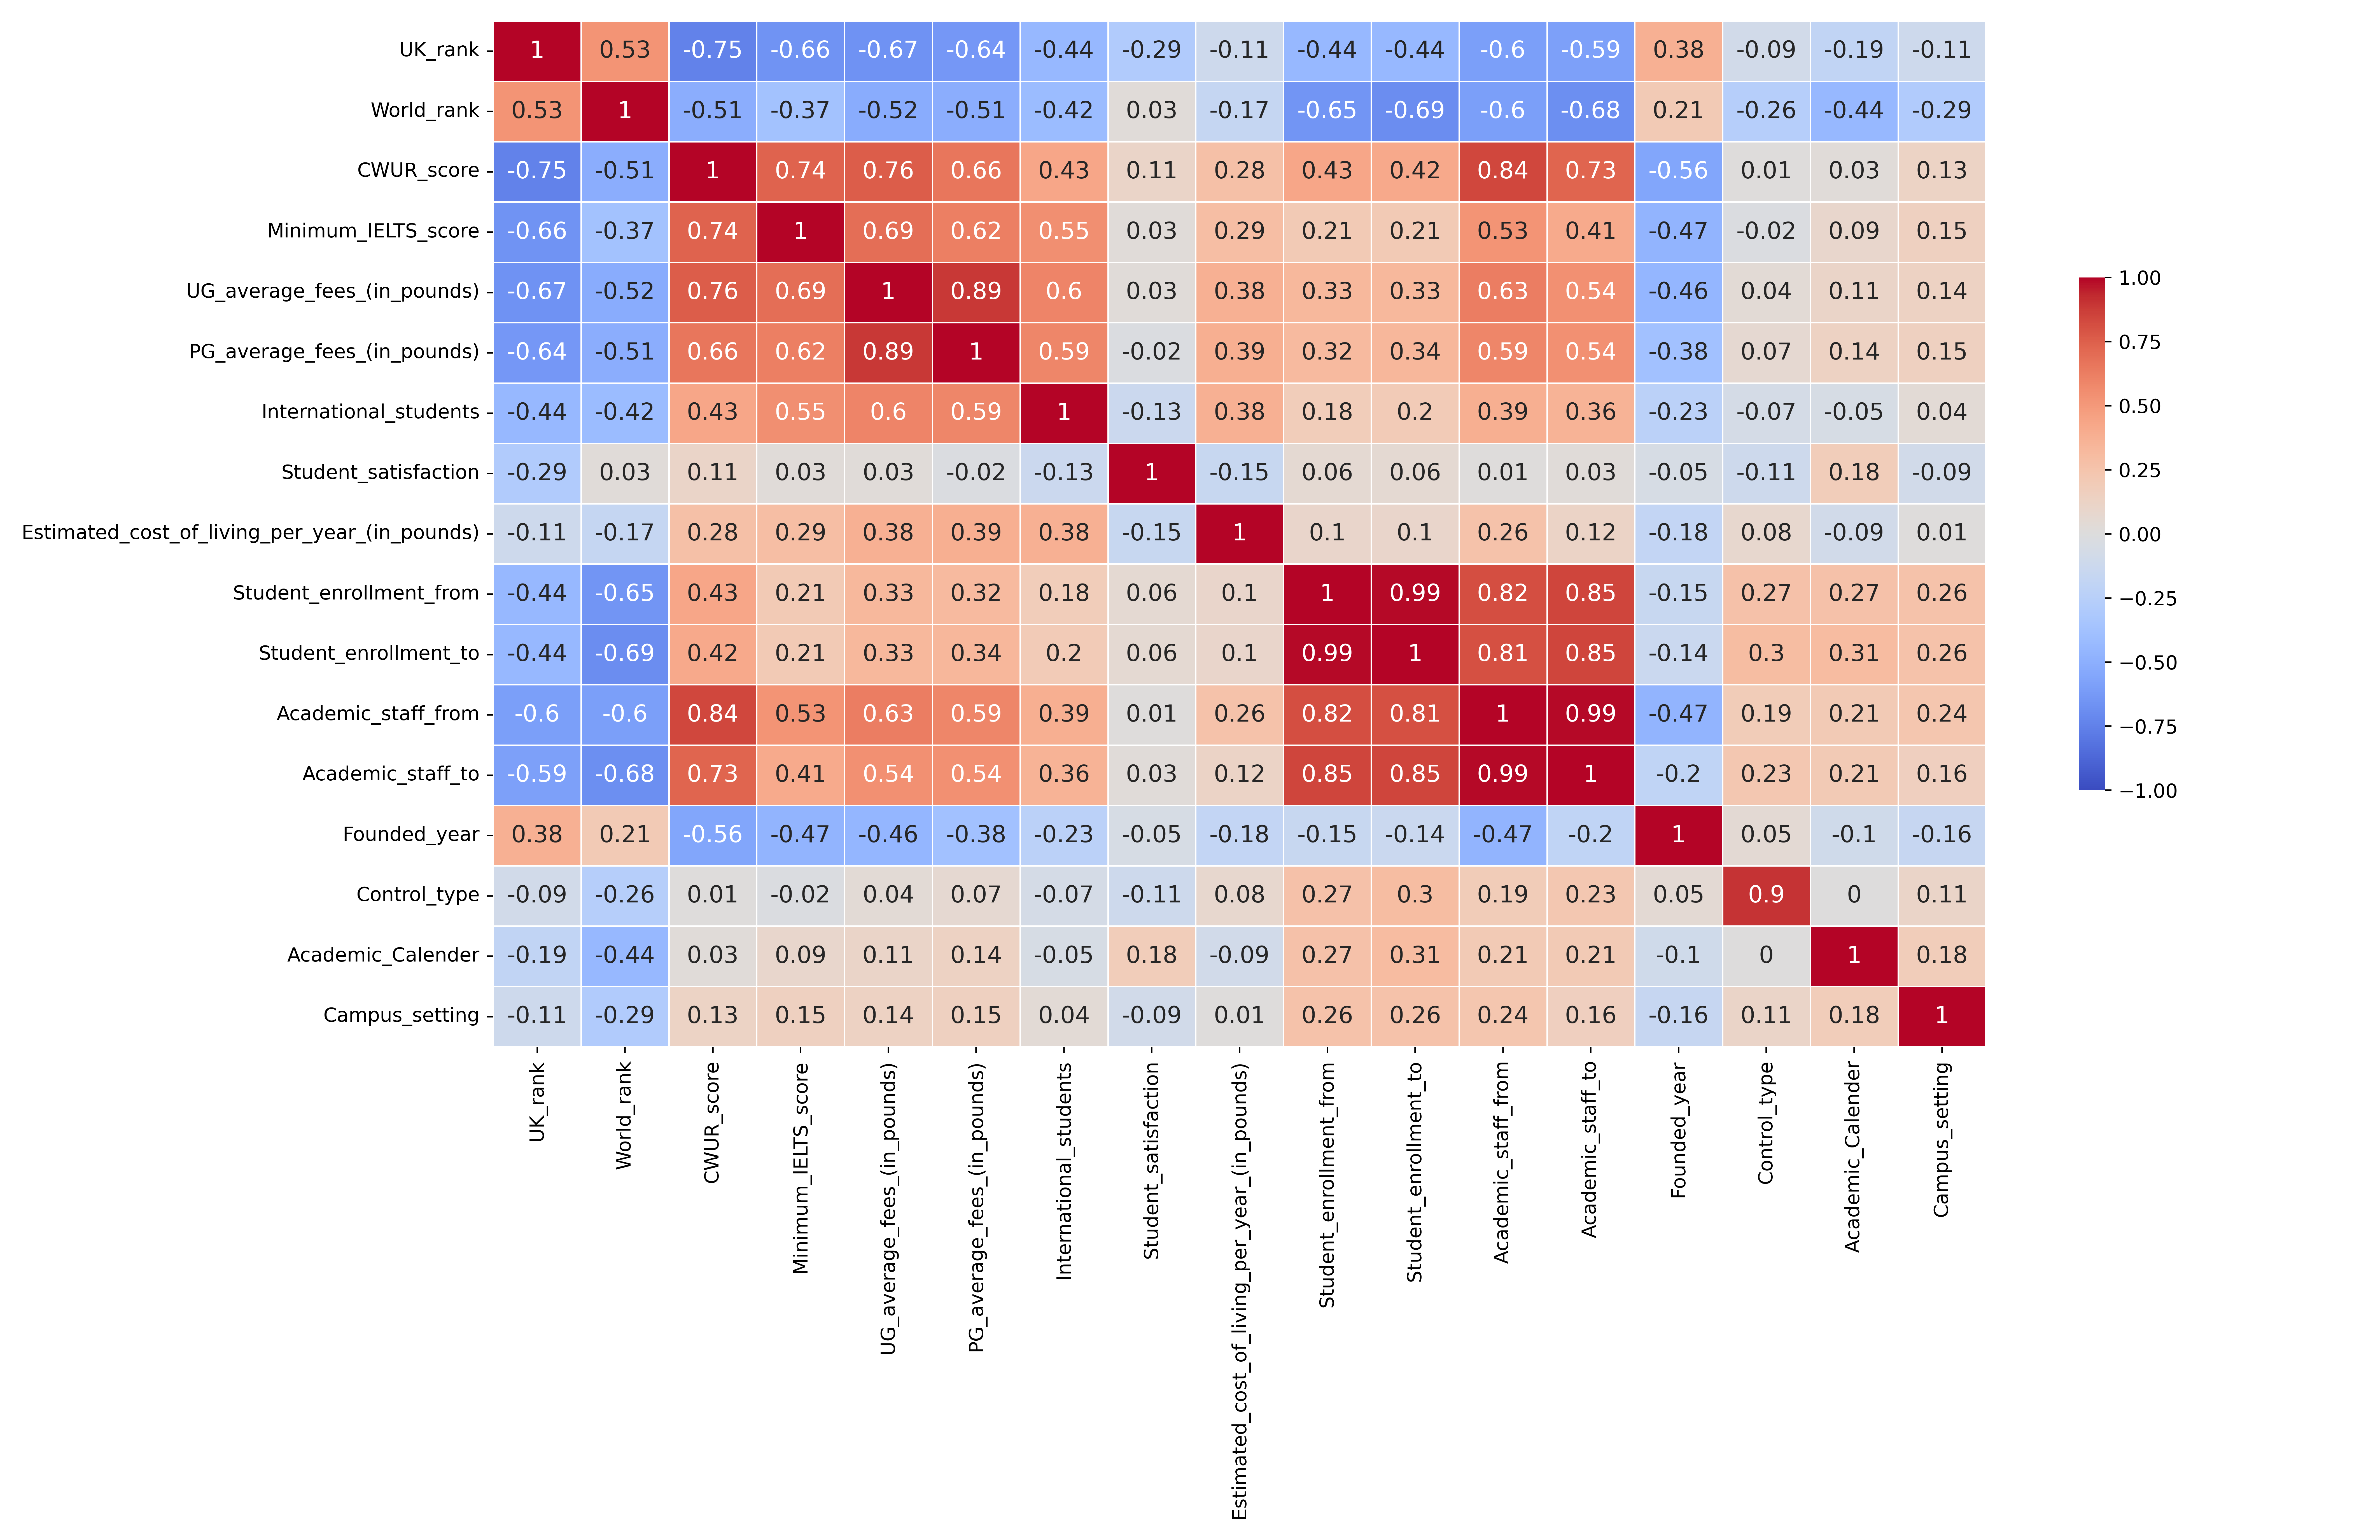
\includegraphics[width=0.91 \textwidth]{figs/correlation_heatmap.png}
    \caption{Correlation heat map}
    \label{fig:corr_heatmap}
\end{figure}
\end{frame}

\begin{frame}{Data Set Analysis 3}
  \vspace{-1cm}
  \begin{figure}
      \centering
      \begin{subfigure}[b]{0.48\textwidth}
          \centering
          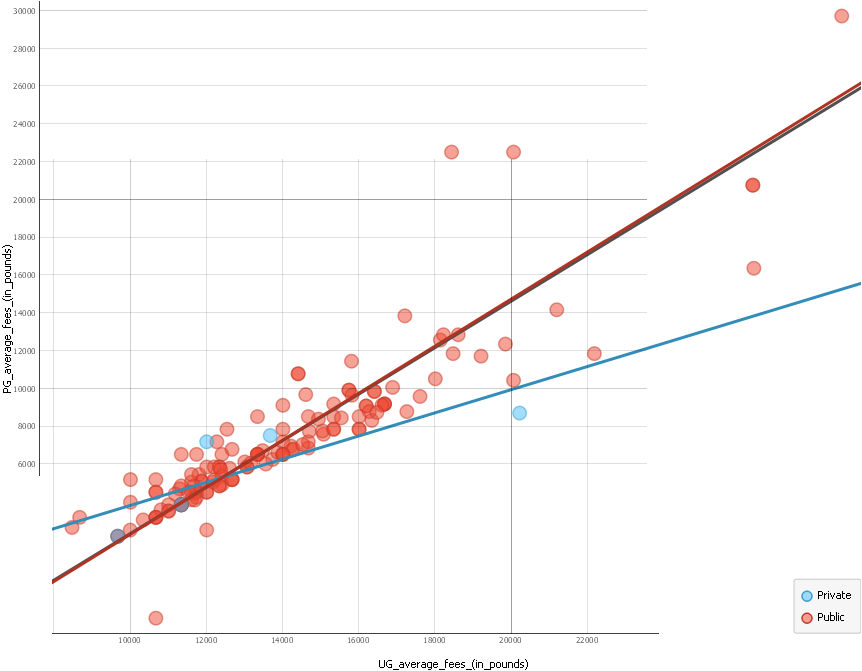
\includegraphics[width=\textwidth, trim={0 0 0 0}, clip]{./figs/scatter_UG_PG_fees_diff.png}
          % \caption{$1$}
          \label{fig:scatter_UG_PG}
      \end{subfigure}
      \hfill
      \begin{subfigure}[b]{0.48\textwidth}
          \centering
          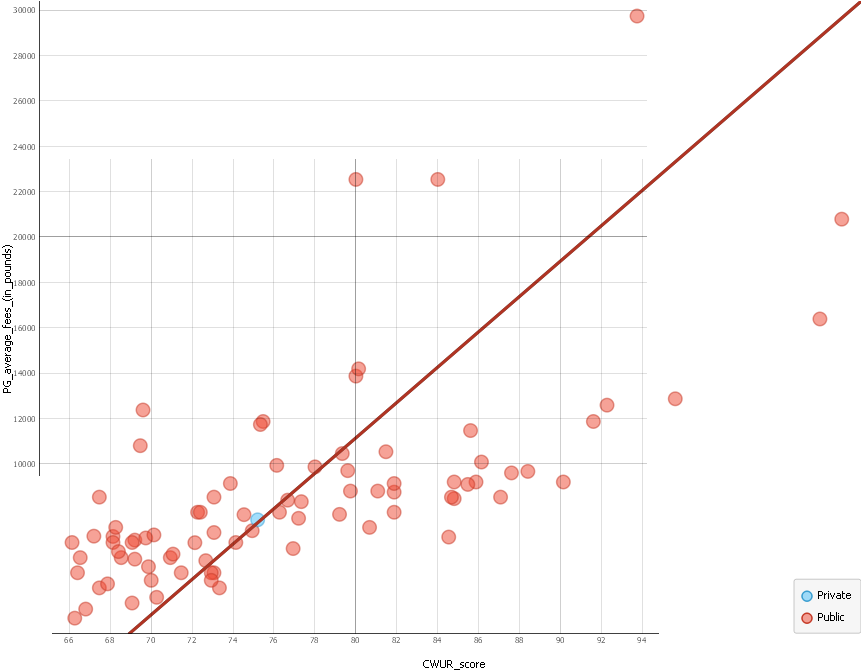
\includegraphics[width=\textwidth, trim={0 0 0 0}, clip]{./figs/scatter_PG_fees_per_CWUR_score.png}
          % \caption{$2$}
          \label{fig:scatter_PG_CWUR}
      \end{subfigure}
      \label{fig:analysis_3}
      \caption{Linear dependency of PG fees, UG fees and CWUR}
    \end{figure}
\end{frame}

\begin{frame}{Data Set Analysis 4}
  \vspace{-1cm}
  \begin{figure}
    \centering
    
    \begin{subfigure}[b]{0.48\textwidth}
      \centering
      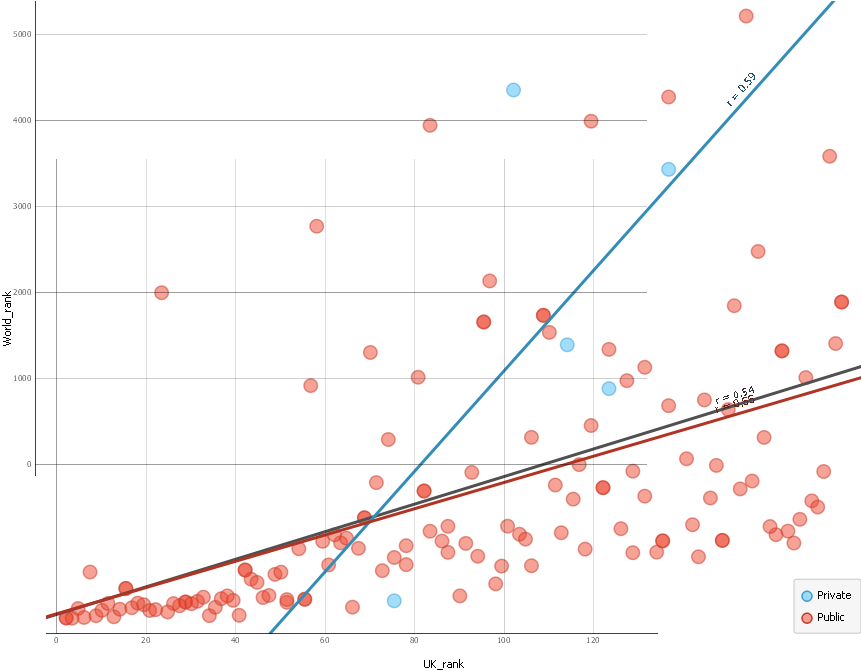
\includegraphics[width=\textwidth, trim={0 0 0 0}, clip]{./figs/scatter_world_rank_per_UK_rank.png}
      % \caption{$3$}
      \label{fig:scatter_World_UK}
    \end{subfigure}
    \hfill
    \begin{subfigure}[b]{0.48\textwidth}
        \centering
        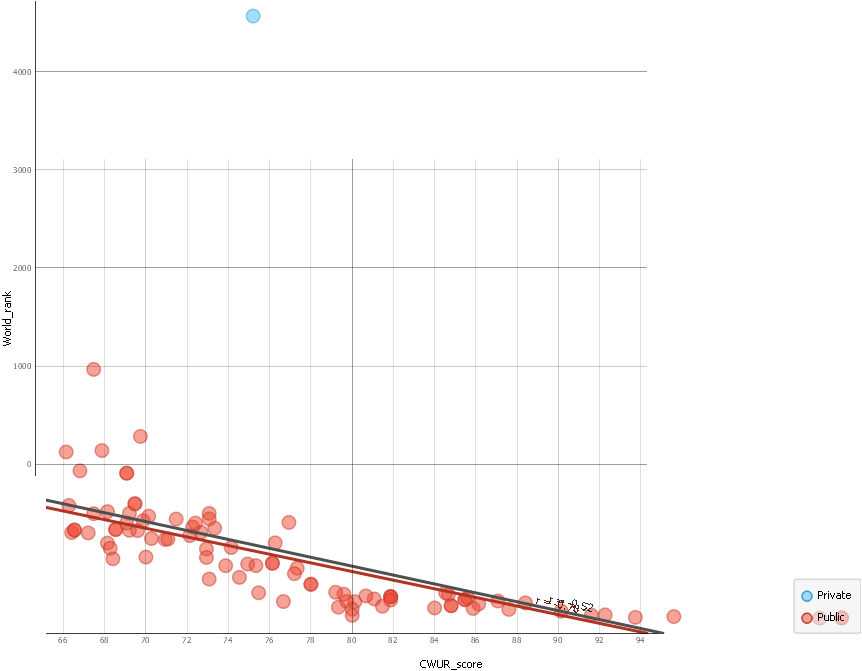
\includegraphics[width=\textwidth, trim={0 0 0 0}, clip]{./figs/scatter_world_rank_per_CWUR.png}
        % \caption{$4$}
        \label{fig:scatter_World_CWUR}
    \end{subfigure}
    
    \caption{Linear dependency of World-rank, UK-rank and CWUR}
    \label{fig:analysis_4}
    \end{figure}
\end{frame}

\begin{frame}{Data Set Analysis 5}
  \vspace{-1.0cm}
  \begin{figure}
      \centering
      
      \begin{subfigure}[b]{0.48\textwidth}
        \centering
        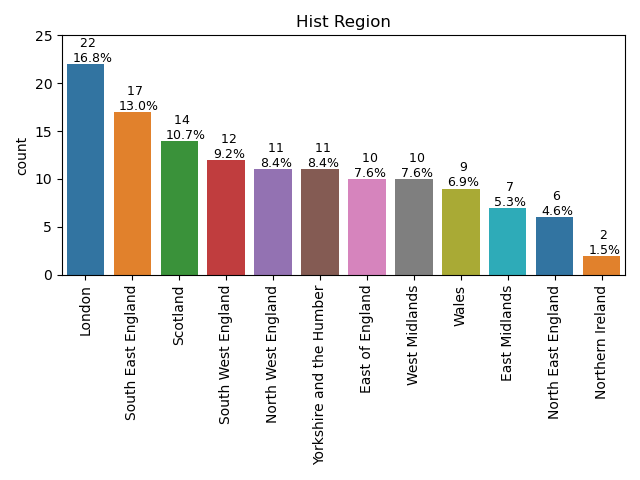
\includegraphics[width=\textwidth, trim={0 0 0 0}, clip]{./figs/bar_hist region.png}
        % \caption{$3$}
        \label{fig:hist_region}
      \end{subfigure}
      \hfill
      \begin{subfigure}[b]{0.48\textwidth}
          \centering
          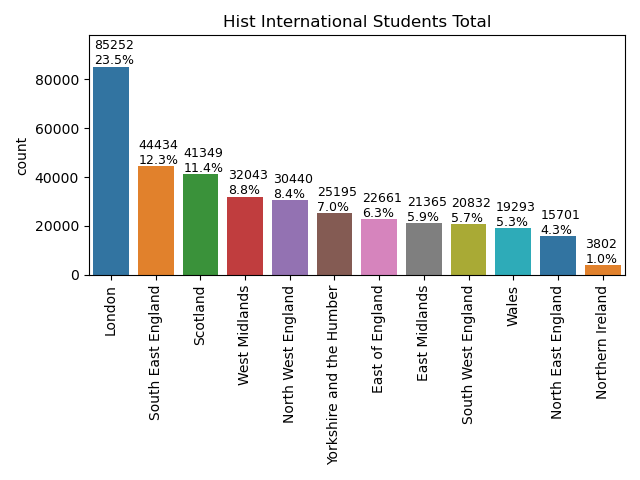
\includegraphics[width=\textwidth, trim={0 0 0 0}, clip]{./figs/bar_hist international students total.png}
          % \caption{$4$}
          \label{fig:hist_international}
      \end{subfigure}
      \hfill
      \vspace{-0.6cm}
      \begin{subfigure}[b]{0.35\textwidth}
        \centering
        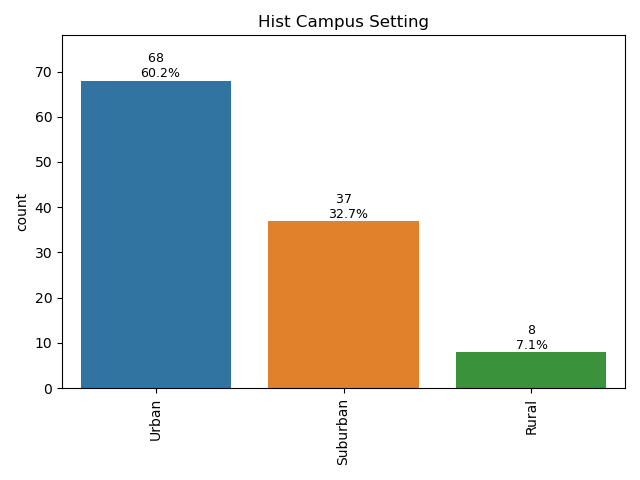
\includegraphics[width=\textwidth, trim={0 0 0 0}, clip]{./figs/bar_hist campus setting.png}
        % \caption{$4$}
        \label{fig:hist_campus}
      \end{subfigure}
      \hfill
      \begin{subfigure}[b]{0.35\textwidth}
        \centering
        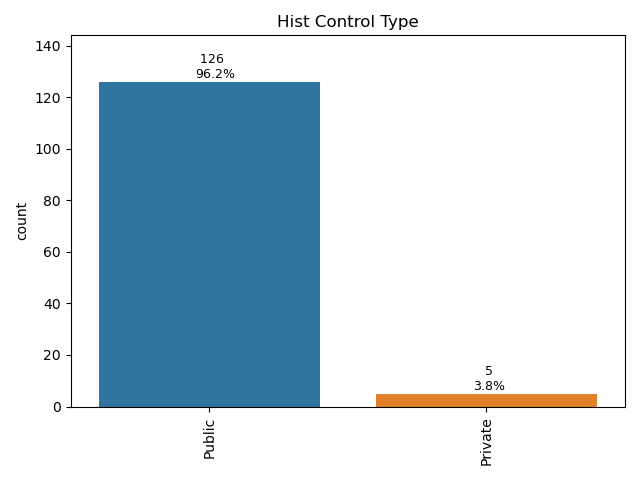
\includegraphics[width=\textwidth, trim={0 0 0 0}, clip]{./figs/bar_hist control type.png}
        % \caption{$4$}
        \label{fig:hist_control_type}
      \end{subfigure}
    \vspace{-1.5cm}
    \caption{Bias}
    \label{fig:analysis_5}
    \end{figure}
\end{frame}

\begin{frame}{Cleaning and Pre-processing}
  \vspace{-1cm}
  \begin{enumerate}
      \item Identification of missing values, split of compound columns, deduplication,
      \item data set split,
      \item missing value imputation,
      \item normalization,
      \item one-hot encoding,
      \item removal of non-numeric columns.
  \end{enumerate}
\end{frame}


\begin{frame}{Imputation (mean, median, mixed)}
  \vspace{-1cm}
  \begin{itemize}
  \item Suspicious values (3 out of 21 columns):
    \begin{table}[h]
      \centering
      \tiny
      \begin{tabular}{l|l|l|lBl}
        Idx & Column                & Suspicious Value & Count & Cleaning Approach \\
        \hline
        3   & Founded\_year         & 9999             & 14    & set NaN \\
        12  & Student\_satisfaction & 0                & 6     & set NaN \\
        14  & Academic\_staff       & over             & 6     & set NaN \\
      \end{tabular}\hfill\
      % \caption{Missing Zero}
      \label{tab:missing_values_zero}
    \end{table}
  \item Missing values (8 out of 21 columns):
    \begin{table}[h]
      \centering
      \tiny
      \begin{tabular}{l|l|lBl|l|l}
        Idx & Column                & NaN & mean    & median  & mixed \\
        \hline
        1   & University\_name      & 14  & dropped & dropped & dropped \\
        3   & Founded\_year         & 28  & mean    & median  & researched online \\
        4   & Motto                 & 17  & dropped & dropped & dropped \\
        7   & CWUR\_score           & 47  & mean    & median  & linear regression on "UK\_rank" \\
        12  & Student\_satisfaction & 6   & mean    & median  & median \\
        14  & Academic\_staff       & 6   & 10'000  & 10'000  & 10'000 \\
        16  & Academic\_Calender    & 26  & mode    & mode    & mode\\
        17  & Campus\_setting       & 18  & mode    & mode    & KNN on "Latitude" and "Longitude"
      \end{tabular}\hfill\
      % \caption{Missing Nan}
      \label{tab:missing_values_nan}
    \end{table}
  \end{itemize}
\end{frame}

\begin{frame}{Training and Evaluation}
  \vspace{-1cm}
  \begin{itemize}
      \item 5-fold cross validation across seeds $[40, 49]$,
      \item 3 subsets of the data set:
        \begin{itemize}
        	\footnotesize
            \item all continuous and categorical columns,
            \item only continuous columns excluding \texttt{Latitude} and \texttt{Longitude}
            \item columns with absolute value of correlation higher than 0.5 with the target variables,
        \end{itemize}
      \item performance evaluation metrics:
      	\begin{itemize}
      		\footnotesize
      		\item MSE, MAE, RMSE, R2 score
		\end{itemize}       
      \item average performance across seeds $[40, 49]$.
  \end{itemize}
\end{frame}

\begin{frame}{Models}
  \vspace{-0.5cm}
  Linear Regression (LR)
  \begin{itemize}
      \item baseline model to assess performance against,
      \item cross validation only for column subsets.
  \end{itemize}
  Fully Connected Neural Network (FCNN)
  \begin{itemize}
      \item 3 architectures with:
        \begin{itemize}
        	\footnotesize
            \item increasing number of hidden layers,
            \item ReLU hidden activation, linear output activation.
        \end{itemize}
  \end{itemize}
\end{frame}

\begin{frame}{Models}
  \vspace{-0.5cm}
  Random Forest (RF)
  \begin{itemize}
      \item grid search parameters:\\
      \begin{itemize}
      	\footnotesize
      	\item max features $[1, 17]$\\
      	\item N estimators $[80, 100]$.
  	\end{itemize}
  \end{itemize}
  Support Vector Regression (SVR)
  \begin{itemize}
      \item grid search parameters:\\
      \begin{itemize}
      	\footnotesize
        \item C (0.005, 0.01, 0.05, 0.1, 0.5, 1, 3, 5)\\
      	\item kernel (linear, rbf)\\
      	\item epsilon (0.0001, 0.0005, 0.005, 0.01, 0.25, 0.5, 1, 5)\\
      	\item gamma (0.0001, 0.001, 0.01, 0.1, 1)
      \end{itemize}
  \end{itemize}
\end{frame}

\begin{frame}{Prediction Performance, Ensemble}
\vspace{-1cm}
\begin{itemize}
    \item no clear best imputation approach,
    \item no clear best subset of columns.
\end{itemize}
\begin{table}[ht!]
\captionsetup{font=scriptsize}
\scriptsize
    \hspace{-0.7cm}
    \begin{tabular}{l|l|l|l|l|l|l}
                 & MSE        & MAE     & RMSE    & R2 score & Columns & Imputation\\
        \hline
        LR       & 3708162.9 & 1408.8 & 1909.6 & 0.3075 & continuous & mixed \\
        FCNN     & 3389145.4 & 1304.6 & 1826.1 & 0.3659 & selected & median \\
        RF       & 3200786.3 & 1192.1 & 1761.7 & 0.4061 & continuous & median \\
        SVR      & 3643681.6 & 1219.7 & 1814.7  & 0.4625 & selected & mixed \\
        \hline
        Ensemble & 2363667.7 & 1108.6 & 1537.3  & 0.5178 & ----- & ----- \\
    \end{tabular}
    \small
    \caption{Average prediction performance across random seeds $[40, 49]$}
    \label{tab:pred_perf}
\end{table}
\end{frame}

\end{document}
